% SLIDE DE RESULTADO SISTEMA MECANICO

\begin{frame}
    \frametitle{Mesa cartesiana no túnel de vento}
        \begin{figure}
            \centering
            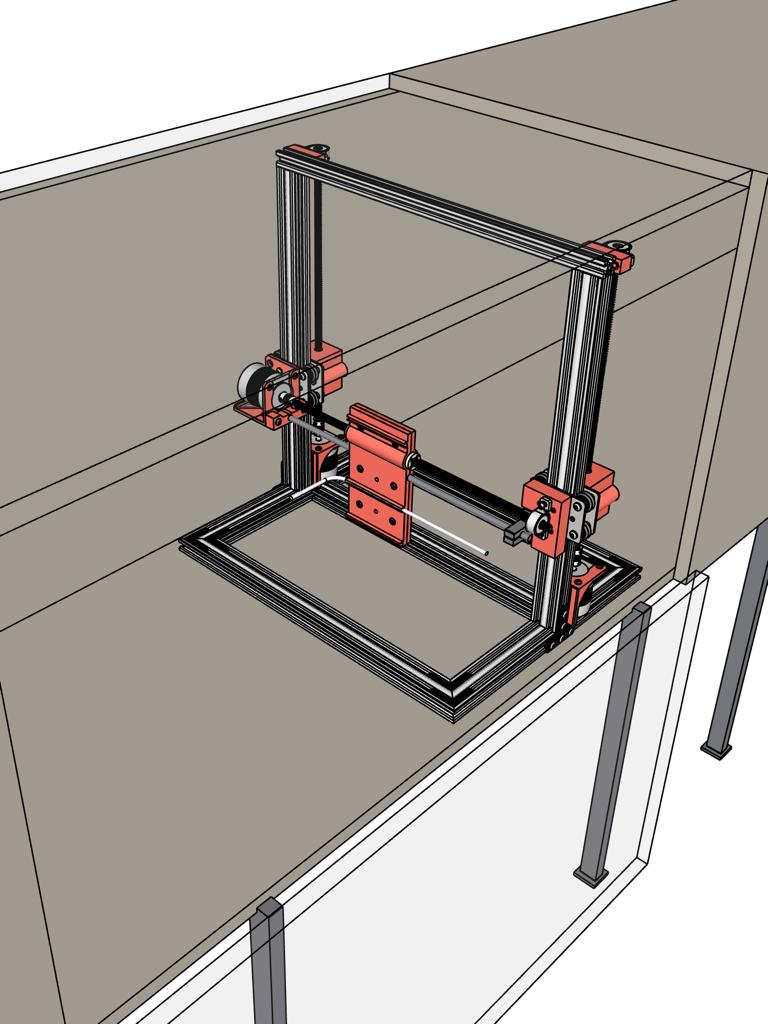
\includegraphics[scale = 0.15]{figuras/mesatunel}
        \end{figure}
\end{frame}

\begin{frame}
    \frametitle{Mesa cartesiana vista frontal}
        \begin{figure}
            \centering
            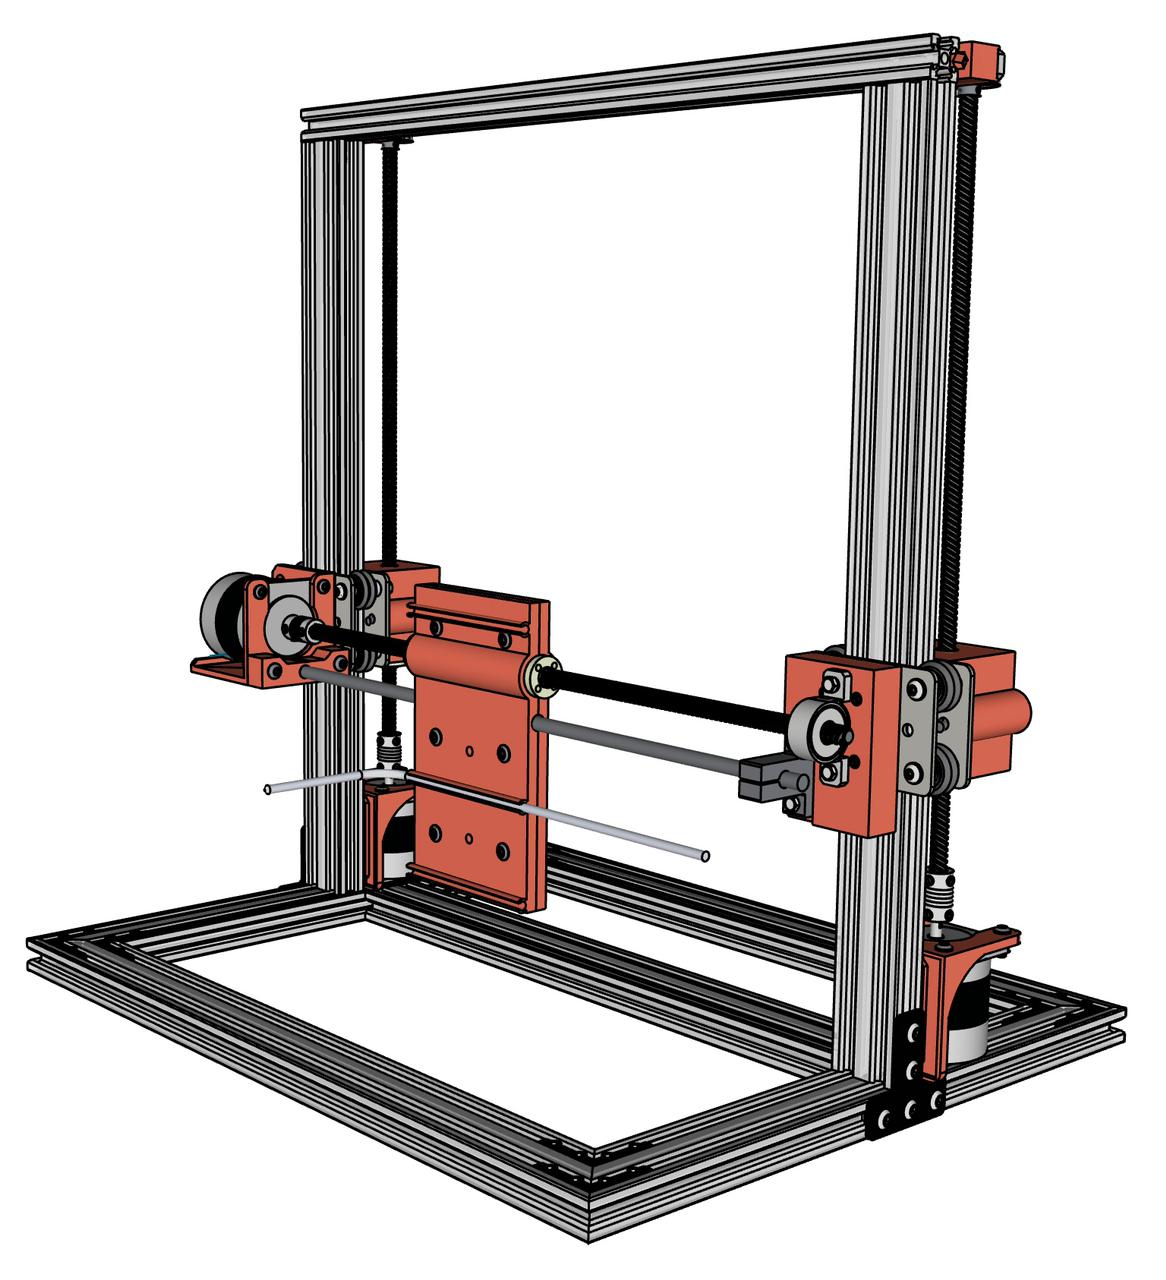
\includegraphics[scale = 0.12]{figuras/mesacartesianaperfil}
        \end{figure}
\end{frame}

\begin{frame}
    \frametitle{Mesa cartesiana vista traseira}  
        \begin{figure}
            \centering
            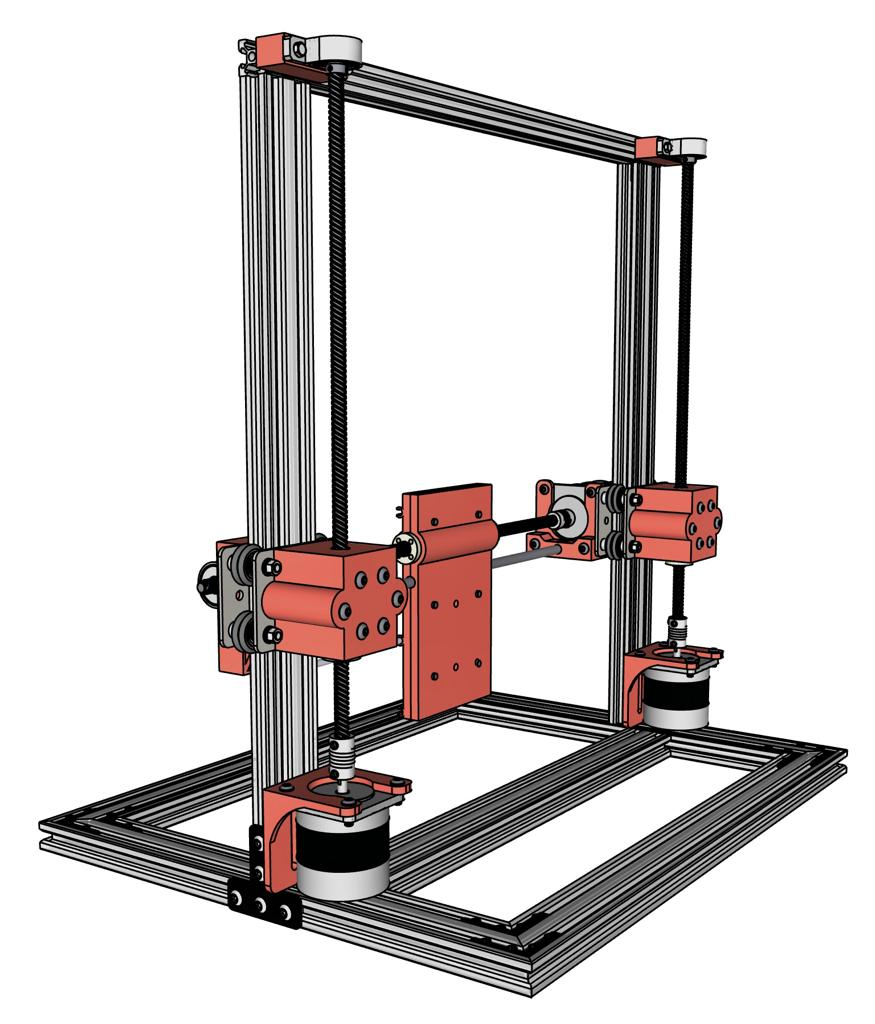
\includegraphics[scale = 0.15]{figuras/mesacartesianaperfiltraseira}
        \end{figure}
\end{frame}

\begin{frame}
    \frametitle{Sistema de posicionamento vertical}  
        \begin{figure}
            \centering
            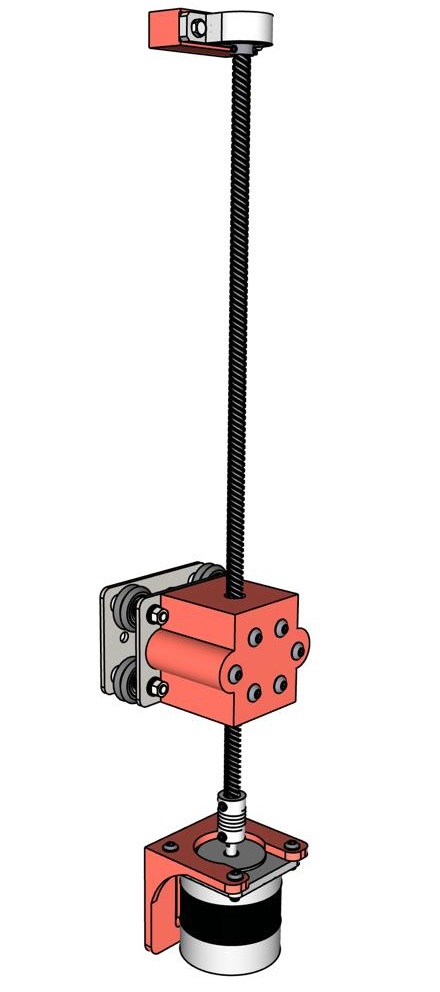
\includegraphics[scale = 0.18]{figuras/sistemaelevacao}
        \end{figure}
\end{frame}

\begin{frame}
    \frametitle{Sistema de posicionamento horizontal}  
        \begin{figure}
            \centering
            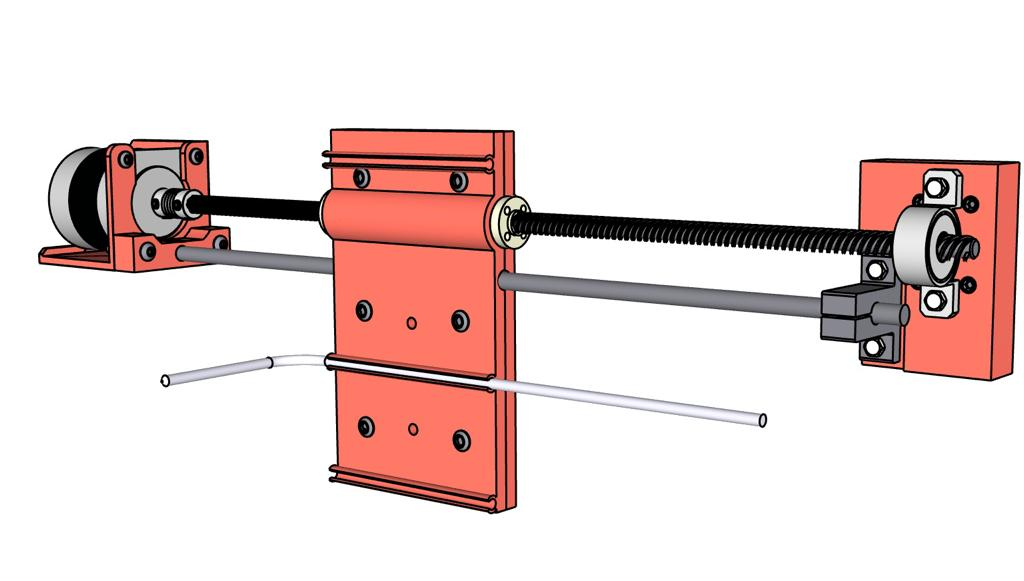
\includegraphics[scale = 0.2]{figuras/sistemaposicionamentohorizontal}
        \end{figure}
\end{frame}

\begin{frame}
    \frametitle{Peças em PLA}
    
    A seguir serão mostradas as peças fabricadas em PLA.

\end{frame}

\begin{frame}
    \frametitle{Suporte do mancal}
        \begin{figure}
            \centering
            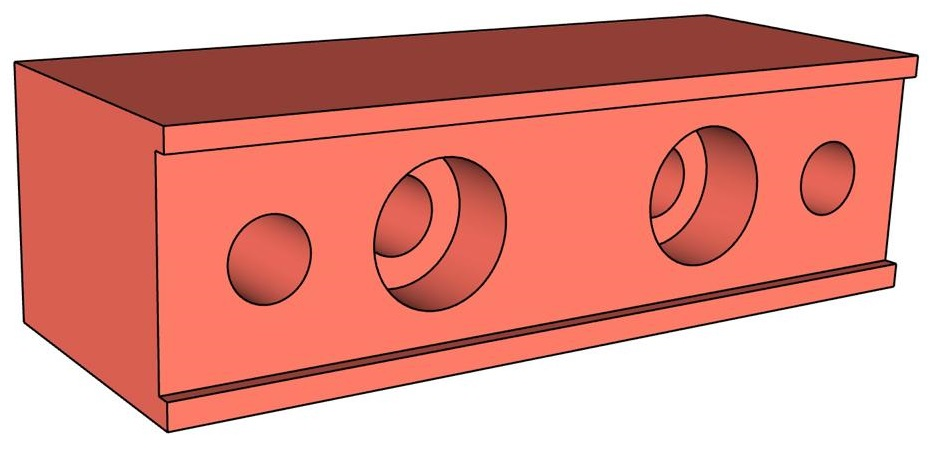
\includegraphics[scale = 0.2]{figuras/ressuportemancal}
            \caption{suportedomancal.stl}
        \end{figure}
\end{frame}

\begin{frame}
    \frametitle{Suporte do motor de passo}
        \begin{figure}
            \centering
            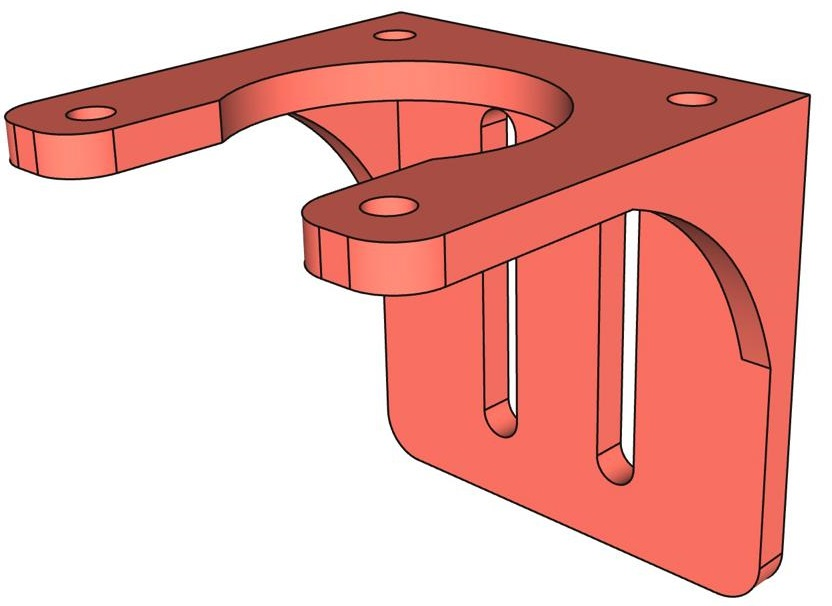
\includegraphics[scale = 0.2]{figuras/ressuportemotorpasso}
            \caption{suportedomotordepasso.stl}
        \end{figure}
\end{frame}

\begin{frame}
    \frametitle{Suporte de elevação}
        \begin{figure}
            \centering
            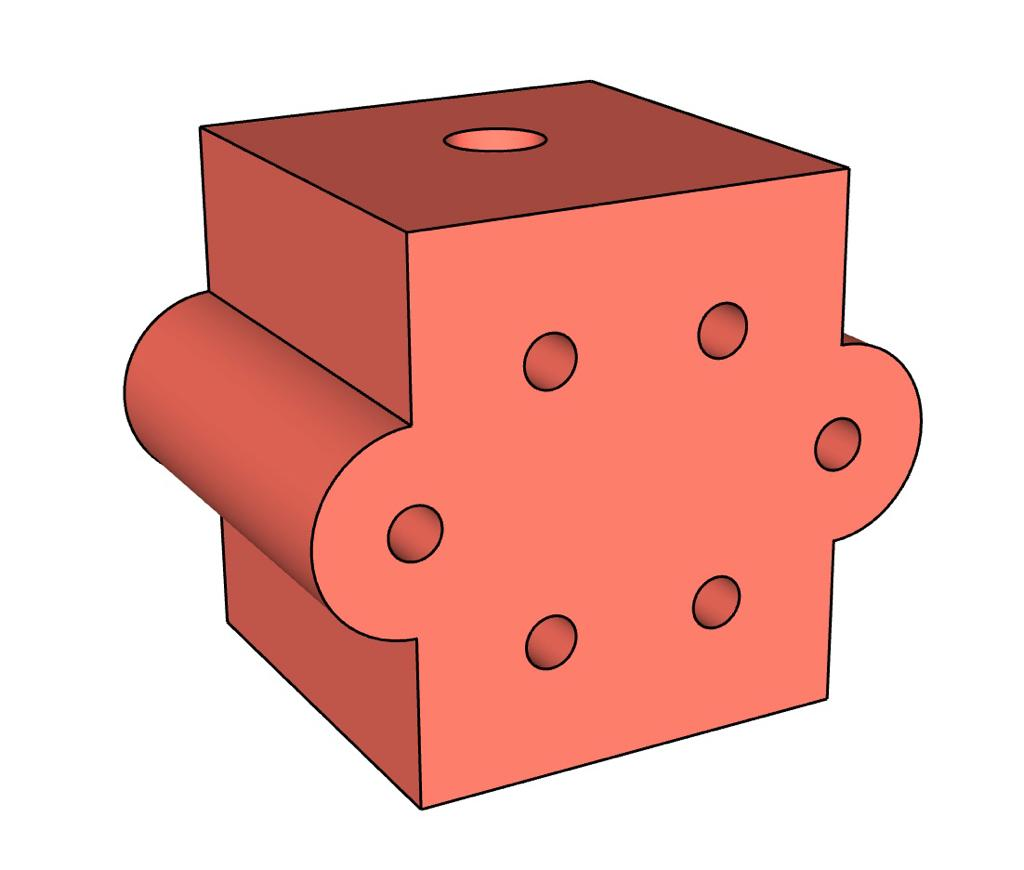
\includegraphics[scale = 0.15]{figuras/ressuporteelevacao}
            \caption{suportedeelevacao.stl}
        \end{figure}
\end{frame}

\begin{frame}
    \frametitle{Suporte do motor horizontal}
        \begin{figure}
            \centering
            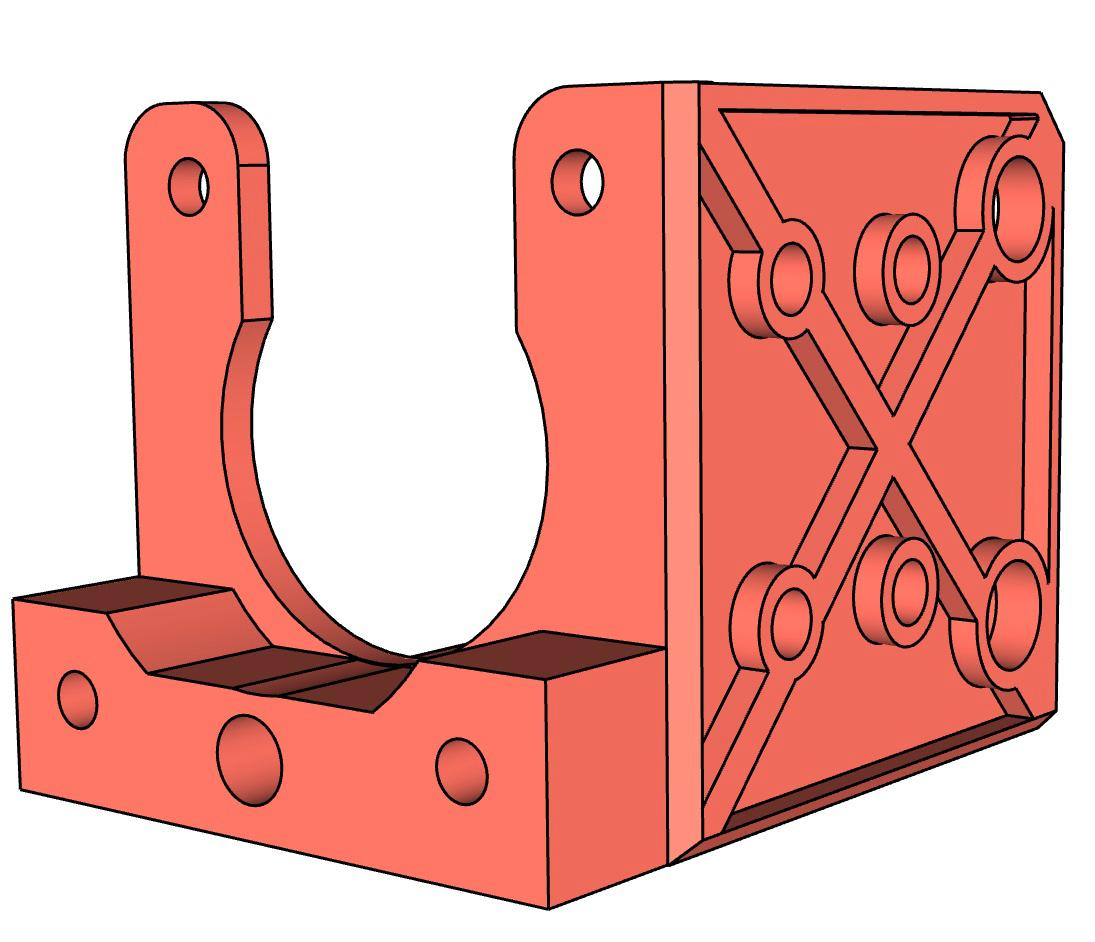
\includegraphics[scale = 0.12]{figuras/ressuportemotorhorizontalf}
            \caption{suportedomotorhorizontal.stl}
        \end{figure}
\end{frame}

\begin{frame}
    \frametitle{Suporte da haste do mancal}
        \begin{figure}
            \centering
            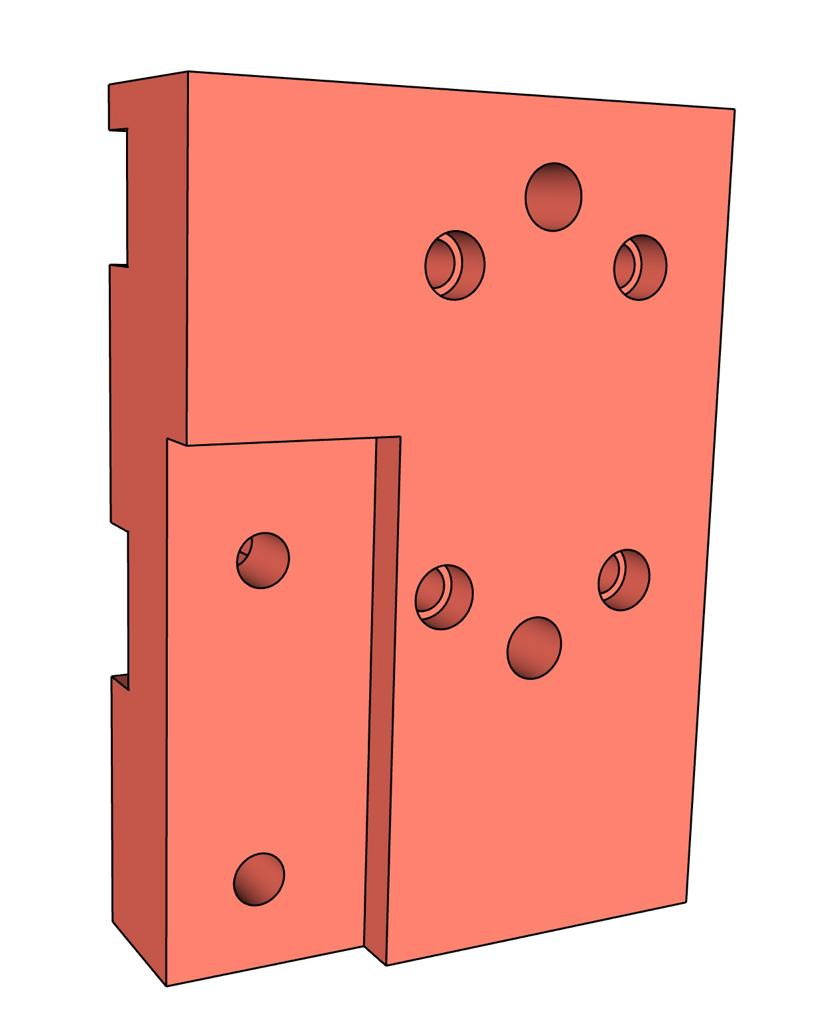
\includegraphics[scale = 0.12]{figuras/ressuportehastemancalf}
            \caption{suportedahastedomancal.stl}
        \end{figure}
\end{frame}

\begin{frame}
    \frametitle{Suporte de serviço}
        \begin{figure}
            \centering
            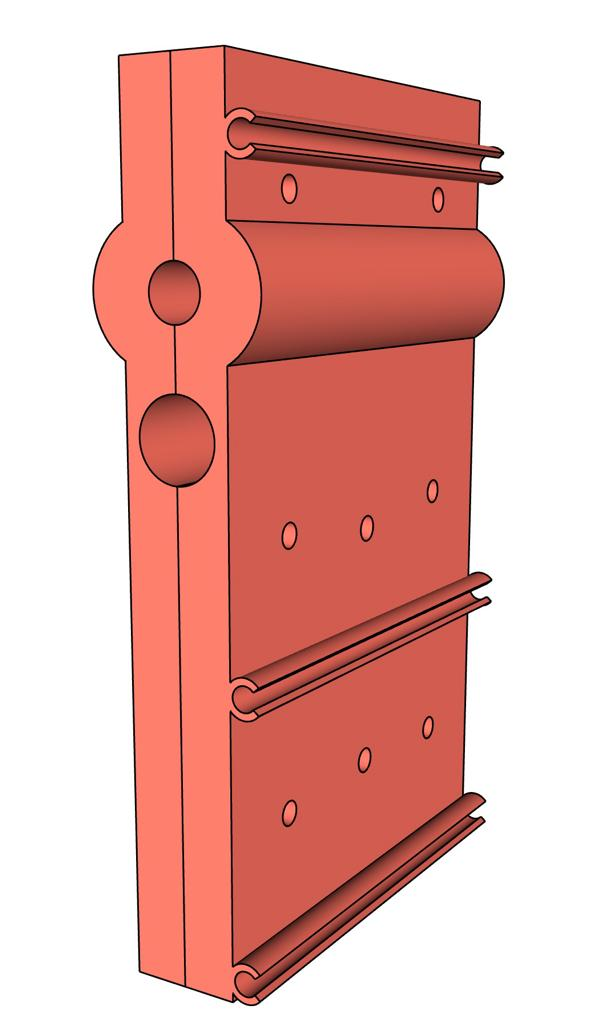
\includegraphics[scale = 0.12]{figuras/ressuporteservicofrontaljunto}
            \caption{suportedeservico.stl}
        \end{figure}
\end{frame}

\begin{frame}
    \frametitle{Suporte de serviço}
        \begin{figure}
            \centering
            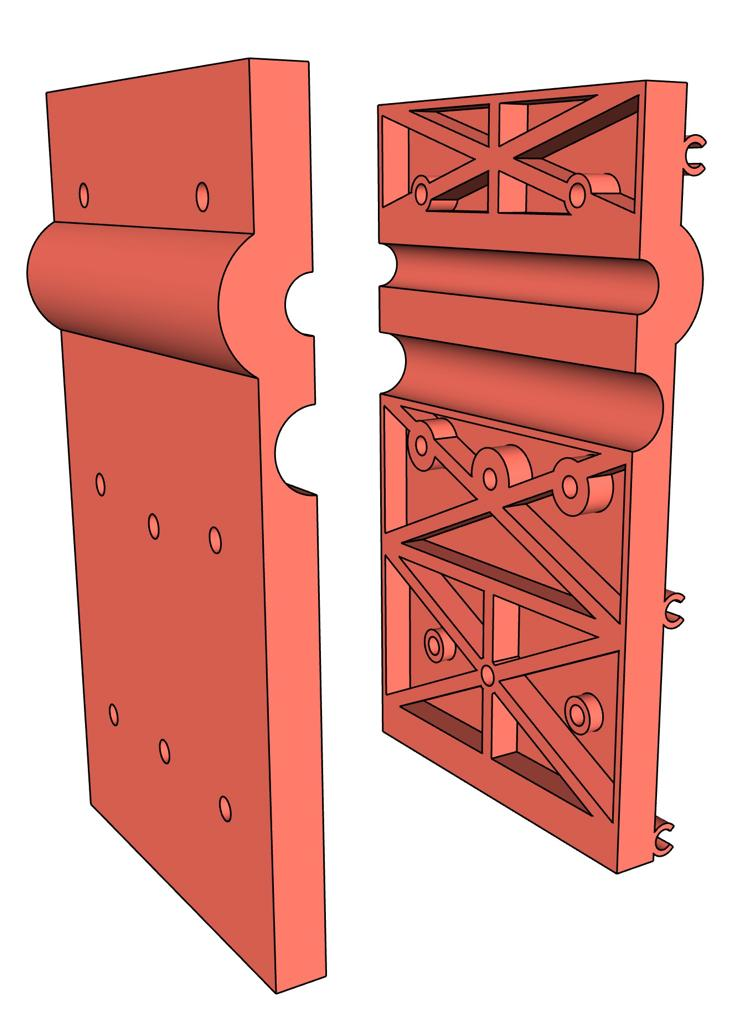
\includegraphics[scale = 0.12]{figuras/ressuporteservicofrontaljuntoseparado}
            \caption{suportedeservico.stl}
        \end{figure}
\end{frame}

\begin{frame}
    \frametitle{Resultado dos cálculos}
    \begin{itemize}
        \item  Para a haste, foi estipulado uma deflexão máxima de $0,05~mm$ resultando em uma força de $22,92106~N$ 
        que equivale aproximadamente $2,3~kg$. Resultando em um coeficiente de segurança de 2,3.
        \item Para a parte do fuso calculou-se a força máxima que ele suportaria erguer, que é de
        306,55~N ou 31,2~kg. 
        \item Considerando a tensão admissível do aço inox 303 que é de 241~MPa com a máxima tensão 
        suportada pelo fuso, na região da raiz do filete, que é de 18~MPa, encontrou-se um fator de
        segurança igual a 13.        
    \end{itemize}
\end{frame}

